\documentclass{beamer}
\usetheme[progressbar=frametitle]{metropolis}           % Use metropolis theme
\usepackage{appendixnumberbeamer}
\usepackage[scale=2]{ccicons}
\usepackage{graphicx}
\usepackage{subfigure}
\usepackage{amsmath} 
\usepackage{amssymb} 
\usepackage{ctable}
\usepackage{array}
\usepackage{microtype} 
\usepackage{hyphenat} 
\usepackage{booktabs}
\usepackage[version=4]{mhchem}
\usepackage{setspace}
\usepackage{paralist}
\usepackage{multirow}
\usepackage[flushleft]{threeparttable}
\usepackage{color}
\usepackage{dcolumn}
\usepackage{adjustbox}
\usepackage{caption}
\usepackage{collectbox}
\usepackage{fontawesome}
\usepackage{listings}




\title{Introduction to R}
\date{\today}
\author{Toni Rodon}
\institute{R introduction, scraping and text analysis (UB) \\ Universitat Pompeu Fabra \\ \faGlobe  \url{www.tonirodon.cat} \\ \faTwitter \href{https://twitter.com/tonirodon}{@tonirodon} }



\begin{document}
  \maketitle


\begin{frame}{Hello everyone}
\begin{itemize}[<+->]
\item Assistant Professor
\item Research Fellow at the LSE
\item Political Behaviour
\item Comparative Politics
\item Historical Political Economy
\item And lots of maps!
 \end{itemize} 
\end{frame}



 \begin{frame}{Digitization}
  \tiny Amat, Francesc; Boix, Carles; Muñoz, Jordi; Rodon, Toni (forthcoming) From Political Mobilization to Electoral Participation: Turnout in Barcelona in the 1930s, The Journal of Politics. 
  \centering
 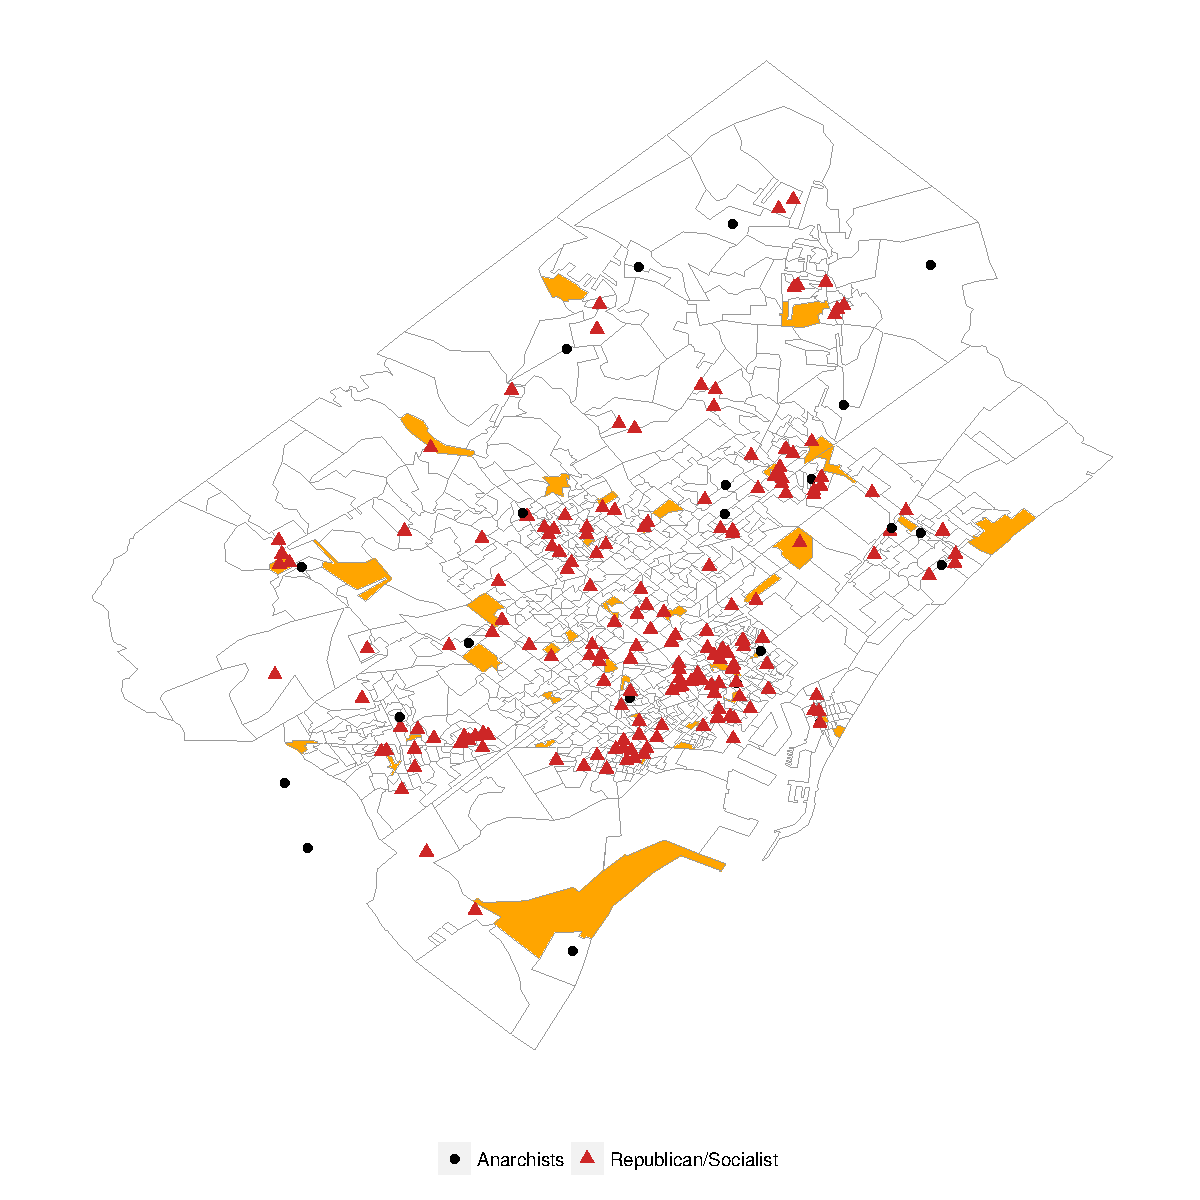
\includegraphics[width=0.7\textwidth]{../Figures/bcn_jop.pdf}
 \end{frame}


\begin{frame}{Who are you?}
\begin{itemize}
\item Name / surname
\item What do you do?
\item Usual data analysis software
\item Haver you ever used R? If yes (or, if no), why? 
 \end{itemize} 
\end{frame}

\begin{frame}{Goal}
\begin{block}{Today} 
The objective of this course is to learn how to use R. \\
We will also learn how to \alert{analyze}, \alert{gather} and \alert{work} with social science data (in R).\\
We will also learn how to not be afraid of using R. \\
After Tuesday's session, most likely you will feel overwhelmed. This is perfectly fine!
\end{block}
\end{frame}

\begin{frame}{History of R}
\begin{itemize}[<+->]
\item R is a powerful environment and programming language for statistical computing and graphics.
\item R was first developed by Robert Gentleman and Ross Ihaka (U of Auckland, NZ) during the 1990s.
\item The language used by R is a ``dialect'' of the S statistical programming language.
\item R version 1.0.0 is released.
\item CRAN package repository features 18,859 available packages.
 \end{itemize} 
\end{frame}


\begin{frame}{Design of the R system}
\begin{itemize}[<+->]
\item The R system is divided into 2 conceptual parts
\begin{itemize}
  \item The ``base'' R system that you download from CRAN
  \item Everything else
  \end{itemize}
 \end{itemize} 
\end{frame}

\begin{frame}{Tutorials}
\begin{itemize}[<+->]
\item Hundreds (thousands!) of tutorials online.
\begin{itemize}
\item An introduction to R \url{https://cran.r-project.org/doc/manuals/r-release/R-intro.html}
\item R for Data Science \url{https://r4ds.had.co.nz/}
\item Quantitative Social Science \url{https://press.princeton.edu/books/hardcover/9780691167039/quantitative-social-science}
\item Quantitative politis with R \url{http://qpolr.com/}
\item Geocomputation with R \url{https://bookdown.org/robinlovelace/geocompr/intro.html}
\item A Business Analyst's Introduction to Business Analytics \url{https://www.causact.com/}
\item Big book of R  \url{https://www.bigbookofr.com/index.html}
\end{itemize}
 \end{itemize} 
\end{frame}


\begin{frame}{Why use R?}
\begin{itemize}[<+->]
\item Data handling, wrangling, and storage
\item Wide array of statistical methods and graphical techniques available
\item Easy to install on any platform and use (and it’s free!)
\item Open source with a large and growing community of peers
\item An enthusiastic community (Stackoverflow, R-help mailing list)
\item Used by New York Times, Facebook, Google, Twitter...
\item Data analysts are in high demand!
 \end{itemize} 
\end{frame}

\begin{frame}{Why did I decide to use R}
\begin{itemize}[<+->]
\item GIS analysis in Stata was almost non-existant
\item Stata graphs are (very) ugly
\item Most top universities mainly use R (or Python)
\item Using R made me think about what I was doing
\item R had functions Stata did not have--scraping, text analysis...
\item It was very annoying to waste my time (paying) or searching for a license key
 \end{itemize} 
\end{frame}


\begin{frame}{Why did I decide to use R}
\begin{itemize}[<+->]
\item I found it very weird to be using a graph scheme in Stata to copy R graphs
\item I don't know anyone transitioning from R to Stata
\item It pays off!
 \end{itemize} 
\end{frame}

\begin{frame}{Things you can do in R}
\begin{itemize}[<+->]
\item Automating your weekly reports (automating tasks)
\item Analyzing data (modeling) or creating your on data model (in a fairly easy way)
\item Creating nicely formatted documents (communicating results)
\item Create interactive maps and export them as a web page
\item Analyze your whatsapp messages (\url{https://cran.r-project.org/web/packages/rwhatsapp/vignettes/Text_Analysis_using_WhatsApp_data.html} or Telegram messages (\url{https://cran.r-project.org/web/packages/telegram/README.html}))
\item Analyze your instagram account (\url{https://github.com/pablobarbera/instaR})
\item Machine learning
\item Create 3-D objects (\url{https://www.tylermw.com/3d-ggplots-with-rayshader/})
 \end{itemize} 
\end{frame}

\begin{frame}{Things you can do in R (II)}
\begin{itemize}[<+->]
\item Extract text from images (\url{https://cran.r-project.org/web/packages/tesseract/vignettes/intro.html} or \url{https://ropensci.org/tutorials/tabulizer_tutorial/})
\item Many new libraries almost every day (\url{https://cran.r-project.org/web/packages/available_packages_by_date.html})
\item It facilitates reproducibility
\item It facilitates replicability
\item Using R you can even order a pizza!
 \end{itemize} 
\end{frame}



\begin{frame}{Disadvantages}
\begin{itemize}[<+->]
\item R is not perfect
\item Steeper learning curve than other languages/softwares
\item R is not always the best tool for everything
\begin{itemize}
  \item Digitize old maps
  \item Some tools for text analysis
  \item etc.
  \end{itemize}
  \item R works for small/medium sized data (me: up to ~8 milion observations)
   \end{itemize} 
\end{frame}


 \begin{frame}{Things you can do in R (III)}
  \centering
 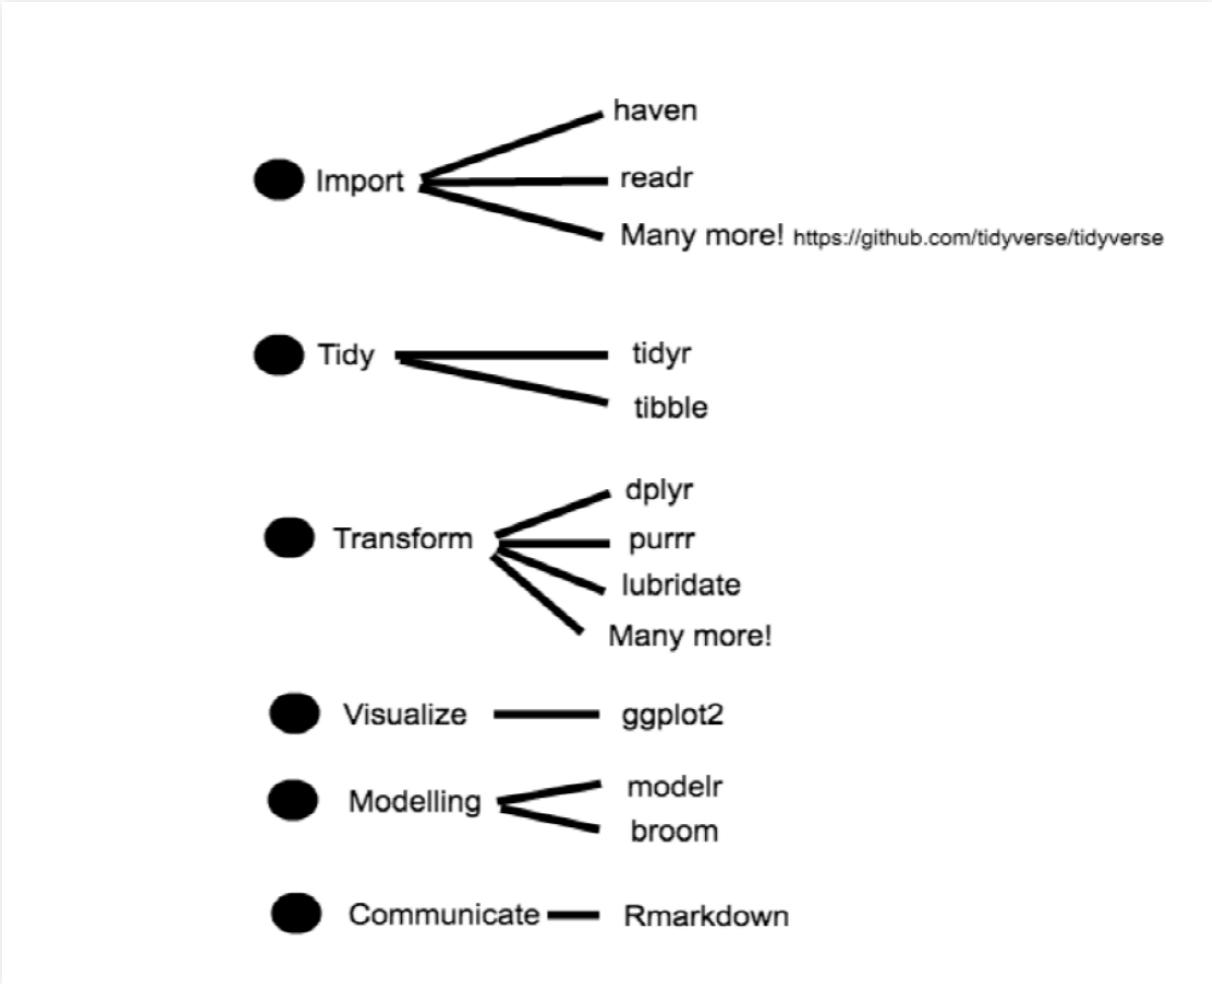
\includegraphics[width=0.7\textwidth]{../Figures/tidyverse.png}
 \end{frame}


 \begin{frame}{Workflow}
 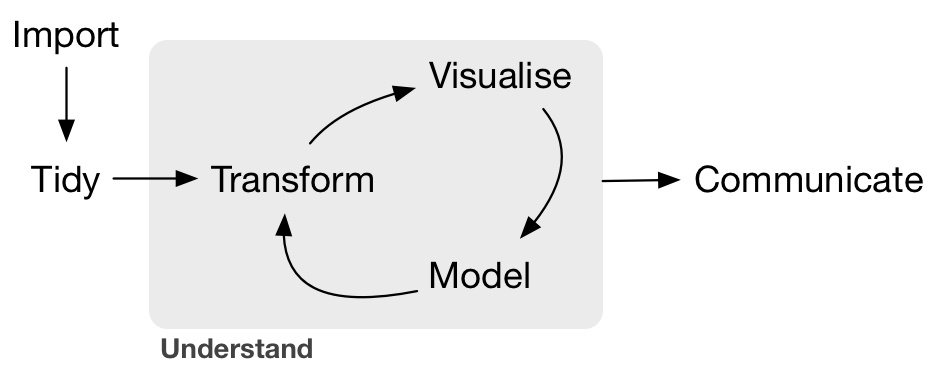
\includegraphics[width=1\textwidth]{../Figures/r4ds_data-science.png}
 \end{frame}


\begin{frame}{Inspirational quotes}
\begin{block}{Hadley Wickham}
The bad news is that when ever you learn a new skill you’re going to suck. It's going to be frustrating. The good news is that is typical and happens to everyone and it is only temporary. You can’t go from knowing nothing to becoming an expert without going through a period of great frustration and great suckiness.
   \end{block} 
\end{frame}

\begin{frame}{Inspirational quotes (II)}
\begin{block}{Kosuke Imai}
One can learn data analysis only by doing, not by reading.
   \end{block} 
\end{frame}


\begin{frame}{Advice}
\begin{itemize}[<+->]
\item Do not use the console, write scripts instead
\item Don't be lazy--don't use the menu!
\item Think before you code
  \item Code is a medium of communication
  \begin{enumerate}
    \item Between you and the computer
    \item Between you and other people
    \item Between you and your future you
 \end{enumerate}
 \item Comment your code
 \item Code should (must!) work from the beginning to the end
   \end{itemize} 
\end{frame}


 \begin{frame}{Future self}
 \centering
 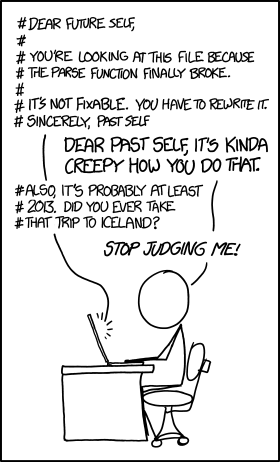
\includegraphics[width=0.4\textwidth]{../Figures/future_self.png}
 \end{frame}

 \begin{frame}{Creating objects}
\begin{itemize}[<+->]
\item R is an object-based language
\item Everything has a name
\item Everything is an object
\item Every object has a class
\item There is no agreement about how to name things. You will likely see variables named snake\_case or SnakeCase or snake\.case
\item There is consensus, however, that variable names can't have blank spaces
   \end{itemize} 
\end{frame}


 \begin{frame}{Other important points}
\begin{itemize}[<+->]
\item R is case-sensitive: Toni\_Rodon is not the same variable or object than toni\_rodon or even than toni\_Rodon
\item An object can only be of one class (not hybrid objects)
\item It is possible to work with multiple objects at the same time (multiple ``datasets'')
\item This means we often need to ``call'' the object (i.e. when using a variable in a dataset) 
   \end{itemize} 
\end{frame}

 \begin{frame}{Examples of R objects}
\begin{itemize}[<+->]
\item character string (i.e. words)
\item number
\item vector
\item matrix
\item list
\item data frame
   \end{itemize} 
\end{frame}

 \begin{frame}{Special values}
\begin{itemize}[<+->]
\item NA: not available, missing (is.na)
\item undefined (is.null)
\item TRUE: logical TRUE (isTRUE)
\item FALSE: logical FALSE (!isTRUE)
   \end{itemize} 
\end{frame}

 \begin{frame}{Dataframes}
\begin{itemize}[<+->]
\item R stores spreadsheets like data in a data frame
\item These are really collections of list vectors of the same length
\item Tip: Create data frames whenever you can
   \end{itemize} 
\end{frame}

 \begin{frame}{Packages or libraries}
\begin{itemize}[<+->]
\item On its own, R can't do all that much
\item To really make use of R's capabilities, we need packages
\item A package bundles together code, data, documentation, and tests
\item We install packages from two sources:
\begin{itemize}
  \item The Comprehensive R Archive Network (CRAN)
  \item Github
\end{itemize}
   \end{itemize} 
\end{frame}

 \begin{frame}{New information on libraries?}
\begin{itemize}[<+->]
\item Twitter.
\item rblogger \url{https://www.r-bloggers.com/}
\item ropensci \url{https://ropensci.org/}
\item github \url{github.com/}
\item \#tidytuesday
   \end{itemize} 
\end{frame}

 \begin{frame}{Today}
\begin{itemize}[<+->]
\item Basics
\item Data wrangling
\item Plotting
\item Univariate analysis
\item Bivariate analysis
\item Multivariate analysis
   \end{itemize} 
\end{frame}

 \begin{frame}{Timetable}
\begin{itemize}[<+->]
\item Please ask for a breack if you feel your brain is melting.
\item I will show some code.
\item You will try to reproduce it--and replicate it.
\item Exercises - and we will go over them together.
   \end{itemize} 
\end{frame}



\begin{frame}{R time}
\begin{block}{R} 
Let's go for it!
\end{block}
\end{frame}



\begin{frame}{Install R}
\begin{itemize}
\item \url{https://github.com/hbctraining/Intro-to-R/blob/master/lessons/01_introR-R-and-RStudio.md}
   \end{itemize} 
\end{frame}

  \maketitle


\end{document}